\documentclass{report}

\usepackage{graphicx}
\usepackage{epstopdf}
\usepackage{amsmath}
\usepackage{amssymb}
\usepackage{amsthm}
\usepackage{algorithm, algpseudocode}
\usepackage{caption}
\usepackage{url}

\newcommand{\rr}[0]{\mathbf{r}}
\newcommand{\xx}[0]{\mathbf{x}}

\begin{document}
\title{Asympototic Statistics of Nodal Domains in Quantum Chaotic Billiards in the Semiclassical Limit}
\author{Kyle Konrad\\
  Dartmouth College\\
  Computer Science Department\\
  Advisor: Alex Barnett}
\date{\today}


\section*{Notation}
$N :=$ number of points sampled

$N \sim h^{-2}$

$B :=$ number of basis functions used in vergini method

$k :=$ wavenumber

$E = k^{2} :=$ energy of eigenfunction

$h :=$ orthogonal spacing between sampled points

$\alpha := k h$

$\Omega \in \mathbb{R}^2$ compact domain

$\Gamma = \partial \Omega$ domain boundary

\chapter{Introduction}
\label{chap:intro}
\section{Motivation}
\label{sec:motivation}
Nodal domains characterize regions of a vibrational surface (e.g. a drum head) that move together. The boundaries between nodal domains, known as nodal line are the regions which do not vibrate at all (Fig. \ref{fig:drum}). Understanding the characteristics of nodal domains has potential applications in musical instruments, mechanical engineering, geophysics, astrophysics, and many other areas dealing with wave behavior \cite{wigman}.

\begin{figure}
  \begin{center}
    \includegraphics[width=\textwidth]{figs/drum/2_3_mode_side_view.eps}
    \caption{A circular vibrational surface with nodal lines shown in black. Nodal domains are regions between black lines}
    \label{fig:drum}
  \end{center}
\end{figure}

The nodal domains studied herein are formulated in terms of quantum mechanical wave functions on Euclidean billiards, a canonical example of quantum chaos. Quantum chaos lies at the intersection of quantum mechanics and chaos theory. The primary signature of chaos in classical systems is a nonlinear (exponential) divergence of paths in the phase space of a system. Quantum mechanics however, is entirely linear and quantum chaos deals with energy eigenfunctions of systems, which are constant in time. Thus chaos in quantum systems is manifest in different ways, one of the most studied being wavefunctions in chaotic domains. Figure \ref{fig:classical_vs_quantum} shows a classical orbit and a quantum eigenfunction on the same billiard.

\begin{figure}
  \begin{center}
    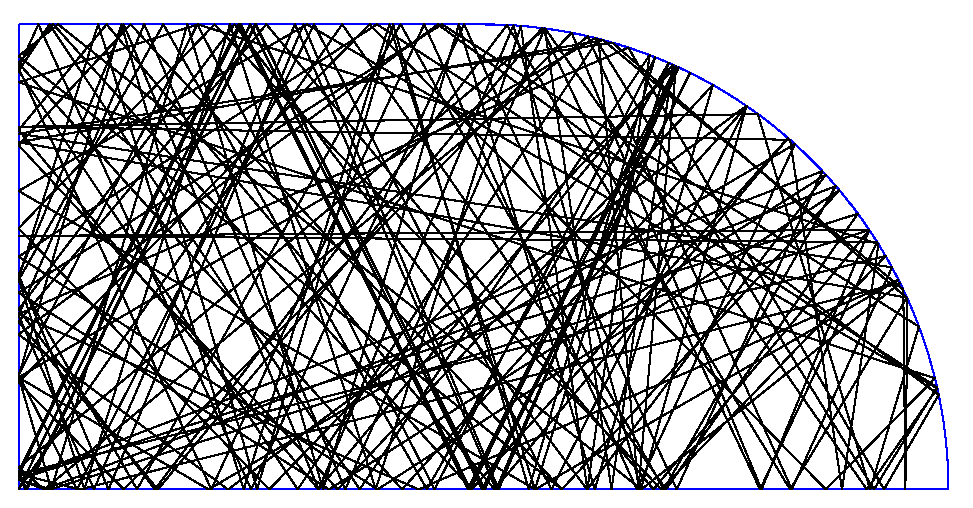
\includegraphics[width=\textwidth]{figs/classical/stadium_orbit.eps}
    \linebreak
    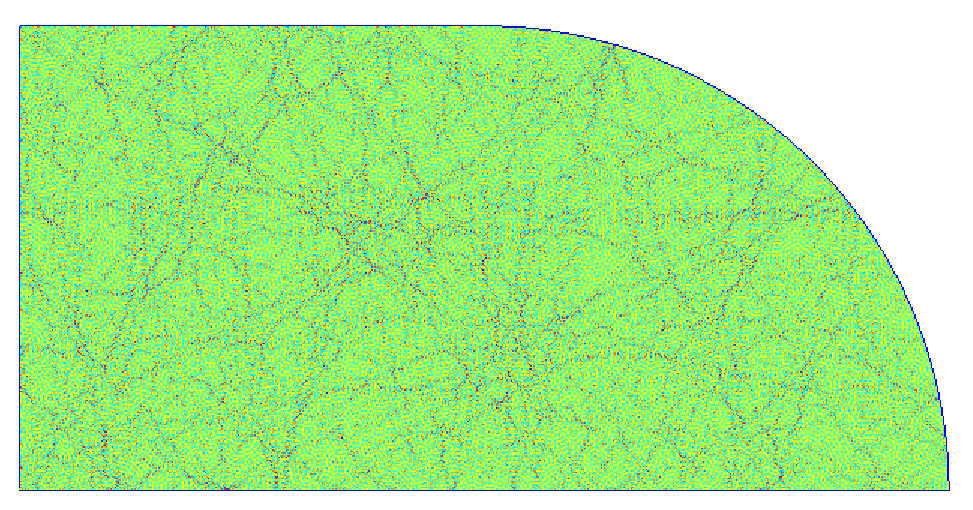
\includegraphics[width=\textwidth]{figs/classical/stadium_eigenfunction.eps}
    \caption{Top: A classical orbit in a billiard; bottom: a quantum eigenfunction in the same billiard}
    \label{fig:classical_vs_quantum}
  \end{center}
\end{figure}

The goal of this project is to numerically test certain conjectures regarding properties of nodal domains in quantum chaotic eigenfunctions in the high energy, or semiclassical, limit. Efficiently testing these conjectures requires solving new computational challenges. We hope these results will enable further mathematical investigation of eigenfunctions and that the tools developed herein may be applied to related problems in experimental mathematics.

\section{Classical Chaos in Billiards}
\label{sec:classical}
A billiard is a compact domain $\Omega \subset \mathbb{R}^{2}$. A billiard defines a map $f(\xx, t): \Omega \times S^{1} \times \mathbb{R} \rightarrow \Omega \times S^{1}$ where $S^{1}$ is the unit circle and $\xx = (q, p) \in \Omega \times S^{1}$ is a point in phase space where $q \in \Omega$ is a position and $p \in S^{1}$ is a momentum, or direction of motion. This map describes the motion of a ball bouncing in the domain $\Omega$.

Chaos in classical systems is characterized by the Lyapunov exponent $\lambda$ of a system, which describes how quickly nearby trajectories diverge. It is computed as the long time ratio of the divergence of two initially close paths:
\[
\lambda = \lim_{t \to \infty} \lim_{\vert \boldsymbol\epsilon \vert \to 0} \frac{1}{t} \frac{\vert f({\bf x_{0}}, t) - f({\bf x_{0}} + \boldsymbol\epsilon, t) \vert}{\vert \boldsymbol\epsilon \vert}
\]
From this definition it follows that
\[
\vert f({\bf x_{0}}, t) - f({\bf x_{0}} + \boldsymbol\epsilon, t) \vert \approx e^{\lambda t} \vert \boldsymbol\epsilon \vert
\]
for small $\boldsymbol\epsilon$ and large $t$. Thus a tiny change $\boldsymbol\epsilon$ in initial conditions produces a change that grows exponentially over time with growth rate $\lambda$. Chaotic systems have a positive Lyapunov exponent and this fact makes it difficult to predict long-term behavior because arbitrarily small errors in measurements of initial conditions eventually become large. As these errors grow to the size of the domain, the position of approaches a uniform distribution over the entire billiard. The property that small subsets of $\Omega$ eventually map to all of $\Omega$ is known as ergodicity (see appendix \ref{sec:ergodicity} for a formal definition).

\section{Quantum Chaos in Billiards}
\label{sec:billiards}
A quantum wave-particle in a billiard $\Omega$ obeys the Schr\"odinger equation
\[
E u(\rr) = - \frac{\hbar^{2}}{2m} \Delta u(\rr) + V(\rr) u(\rr)
\]
Where $\Delta = \nabla^{2} = \frac{\partial^{2}}{\partial x^{2}} + \frac{\partial^{2}}{\partial y^{2}}$ is the Laplacian differential operator in two dimensions. Setting $\hbar = 2m = 1$ and $V(\rr) = 0$ for $\rr \in \Omega$ while enforcing Dirichlet boundary conditions $u(\rr) = 0$ for $\rr \in \Gamma = \partial \Omega$ simplifies this to the Helmholtz equation
\begin{equation}
\label{eq:helmholtz}
\begin{cases}
(\Delta + k^{2})u(\rr) = 0 & \text{if } \rr \in \Omega\\
  u(\rr) = 0 & \text{if } \rr \in \Gamma
\end{cases}
\end{equation}
where $k^{2} = E$ is the energy of the eigenfunction $u(\rr)$ and corresponds to the kinetic energy of the quantum wave-particle.

We focus our investigation on two billard shapes: the generalized rectangular Sinai billiard and the Stadium billiard. In both cases we desymmetrize the billard shapes by considering only a quarter of the full shape. This restricts our basis set to functions that are odd as a function of x and y, i.e., $f(-x,y) = f(x,-y) = -f(x,y)$. The desymmetrized billiards are shown in figure \ref{fig:billiards}

\begin{figure}
  \begin{center}
    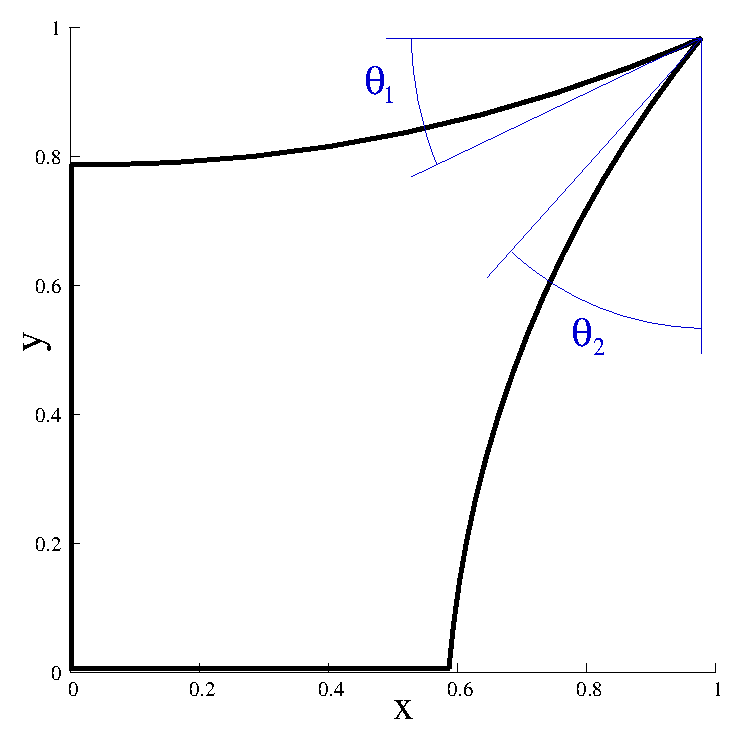
\includegraphics[width=0.3\textwidth]{figs/domains/qugrs_fig.eps}
    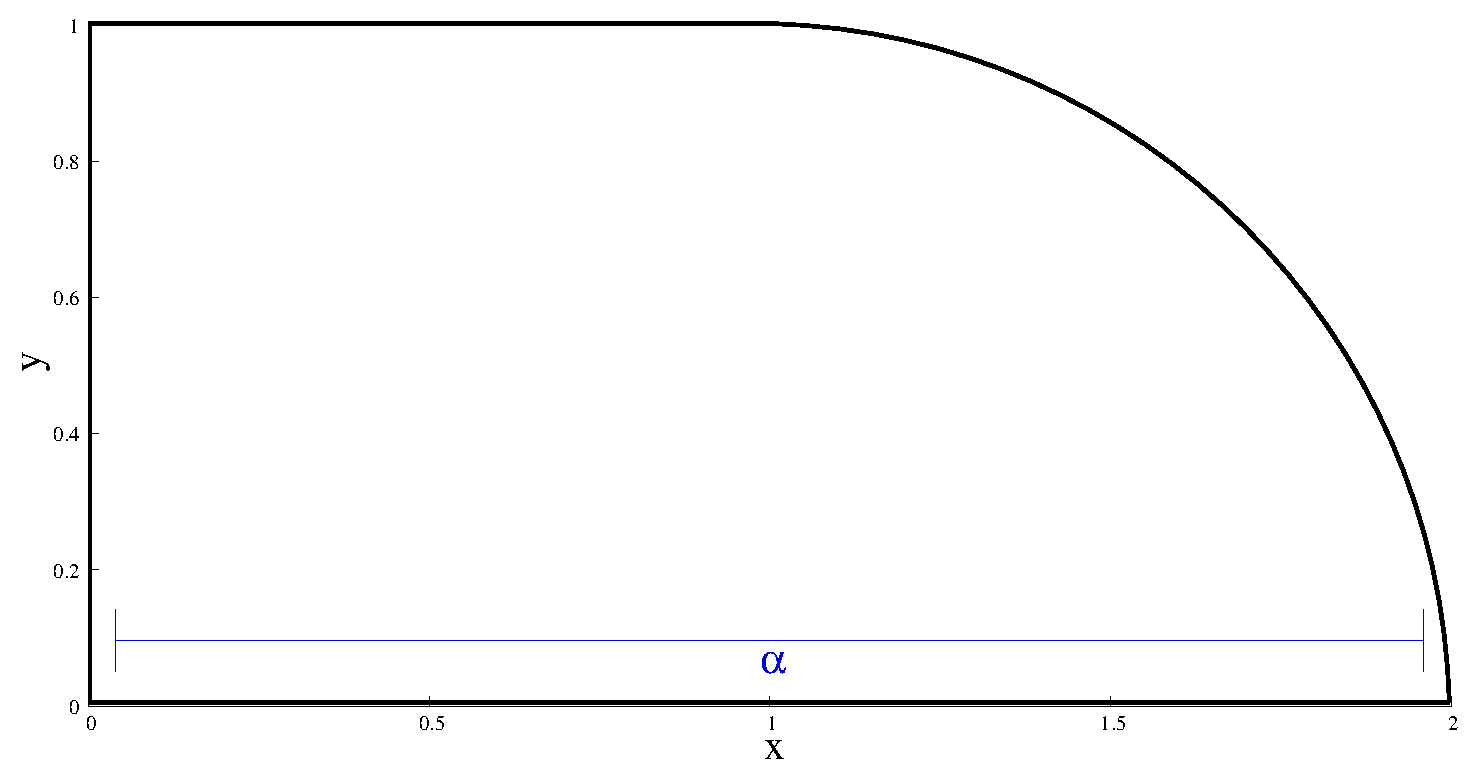
\includegraphics[width=0.6\textwidth]{figs/domains/qust_fig.eps}
    \caption{Left: quarter generalized rectangular Sinai billiard; right: quarter stadium billiard}
    \label{fig:billiards}
  \end{center}
\end{figure}

The Sinai billiard is constructed from circular arcs that meet at $(1,1)$ and is parameterized by two angles, $\theta_{1}$ and $\theta_{2}$, the angles from horizonal and vertical, respectively, of the arcs at $(1,1)$. The Sinai billiard is said to demonstrate ``hard chaos'' becase there are no stable orbits.

The stadium billiard is construced from a rectangular region and a quarter circle and is parameterized by the the horizontal length of the billiard $\alpha$. The stadium billiard contians neutrally stable orbits, specifically those with vertical momentum in the rectangular region. Neutrally stable orbits have zero Lyapunov exponent but any perturbation will cause them to have positive Lyapunov exponenet. The existence of such orbits implies that the stadium does not demonstrate hard chaos but because these orbits occupy a measure zero subset of phase space, the stadium still demonstrates chaotic properties.

\section{Percolation Model}
Bogomolny and Schmit \cite{bogomolny} have argued that nodal domains of random functions (which are considered an accurate proxy for eigenfunctions of chaotic systems) can be modeled by nodal domains of a percolation model. Their percolation model is formed by creating a checkerboard of positive and negative regions with a grid size given by the average spacing of zeros of random functions along a particular axis. This checkerboard pattern can be realized as an eigenfunction $\bar{u}(x,y) = sin(\frac{kx}{\sqrt{2}})sin(\frac{ky}{\sqrt{2}})$ of a square billiard $\Omega = [0,1]^{2}$. A random eigenfunction can be modelled as this mean eigenfunction $\bar{u}(x,y)$ plus another term representing deviation from the mean $u(x,y) = \bar u(x,y) + \delta u(x,y)$. The deviation term $\delta u(x,y)$ is modelled by perturbing each nodal line crossing by connecting two diagonal regions (Fig. \ref{fig:percolation}). The decision of which nodal domains to connect is made randomly with equal probability for either possibility.

\begin{figure}
  \begin{center}
    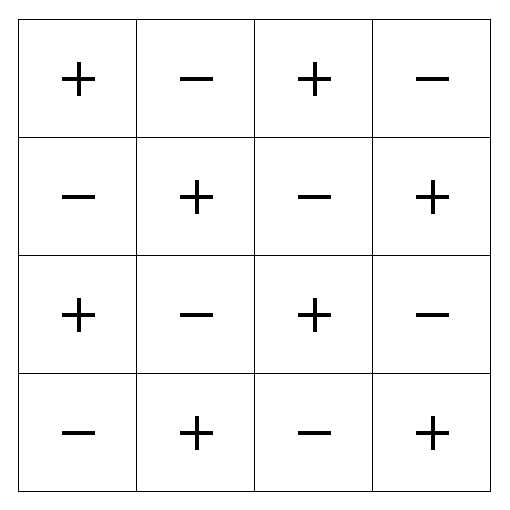
\includegraphics[width=0.4\textwidth]{figs/percolation/checkerboard.eps}
    \hspace{1 cm}
    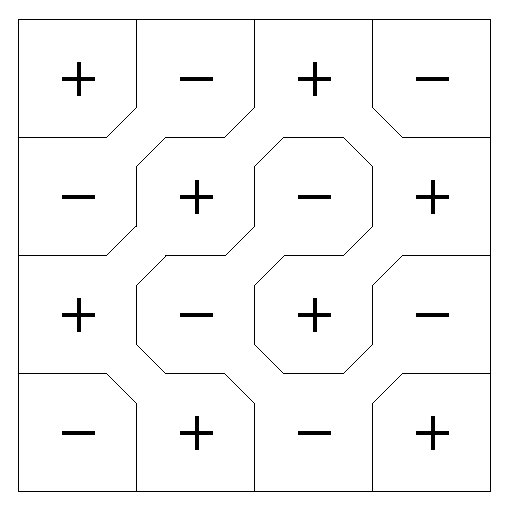
\includegraphics[width=0.4\textwidth]{figs/percolation/perturbed.eps}
    \caption{Left: checkerboard pattern; right: perturbed checkerboard pattern}
    \label{fig:percolation}
  \end{center}
\end{figure}

Bogomolny and Schmit apply results from graph theory and statistical physics to compute the distribution of nodal domains in this percolation model. These results form the two primary conjectures we wish to test numerically.

\newtheorem{conj}{Conjecture}
\begin{conj}[Mean of Nodal Domain Count]
  The number of nodal domains $\nu(E)$ in a quantum chaotic eigenfunction with energy $E$ is normally distributed with mean
  \begin{equation}
    \label{eq:mean_prediction}
    \frac{\bar{\nu}(E)}{\bar{N}(E)} = \frac{3 \sqrt{3} - 5}{\pi} \approx 0.0624
  \end{equation}
\end{conj}

\begin{conj}[Variance of Nodal Domain Count]
  The number of nodal domains $\nu(E)$ in a quantum chaotic eigenfunction with energy $E$ is normally distributed with variance
  \begin{equation}
    \label{eq:variance_prediction}
    \frac{\sigma^{2}(\nu(E))}{\bar{N}(E)} = \frac{18}{\pi^{2}} + \frac{4 \sqrt{3}}{\pi} - \frac{25}{2 \pi} \approx 0.0502
  \end{equation}
\end{conj}  

In both conjectures, $\bar{N}(E)$ is the mean number of eigenfunctions with energy less than $E$ which is given by Weyl's law \cite{garabedian} to be
\[
\bar{N}(E) = \frac{\vert \Omega \vert E}{4 \pi}
\]

Bogolmony and Schmit also obtain a prediction for the distribution of areas of nodal domains

\begin{conj}[Area of Nodal Domains]
  The area $s$ of nodal domains in a quantum chaotic eigenfunction follows the distribution
  \begin{equation}
    \label{eq:area_prediction}
    f(s) \propto s^{-\tau}
  \end{equation}
  where $\tau = \frac{187}{91}$
\end{conj}

\chapter{Methods}
\section{Scaling Method}
\subsection{Theory}
Vergini and Saraceno \cite{vergini} developed a method of computing high energy eigenfunctions of chaotic billiards using a scaling method. The method simultaneously finds all eigenfunctions $\phi_{i}(\rr)$ with energy in a given window $[E - \Delta E, E + \Delta E]$ for some $E = k^{2}$ by scaling each eigenfunction. The scaled eigenfunctions $\chi_{i}(k, \rr)$ are computed as
\[
\chi_{i}(k, \rr) = \phi_{i} \left( \frac{k}{k_{i}} \rr \right) = \phi_{i} \left( \rr + \frac{\omega_{i}}{k_i} \rr \right)
\]
where $\omega_{i} = k - k_i$. This scaling causes all eigenfunctions to fall approximately in a linear subspace of a single basis set $\left\{ \xi_{l} \right\}_{l=1}^{B}$, that is
\[
\chi_{i}(k, \rr) = \sum_{l=1}^{B} X_{li} \xi_{l}(k, \rr) + \epsilon_{i}(\rr)
\]
where $\epsilon_{i}(\rr) \ll 1$ for sufficiently large $B$, the number of basis functions used. Values of $B$ of approximately $1.5 \frac{k \vert \Gamma \vert}{\pi}$ have been shown to produce $\epsilon < 10^{-4}$. This single basis set provides a significant efficiency gain over prior methods because many eigenfunctions can be found by solving a single linear system.

The choice of basis functions $\xi_{l}(k, \rr)$ depend on the billiard shape being used. For the quarter generalized rectangular Sinai billiard the basis set consists of irregular Bessel functions (which satisfy $(\Delta + k^2)\xi_{l}(k, \rr) = 0$) placed along $\Gamma^{+}$, the set of points ouside $\Omega$ whose nearest distance to $\Gamma$ is $D$ where $kD$ is taken to be $7$ so that $D$ is appriximately one wavelength. For the quarter stadium, the basis set is plane waves with orientations evently spaced around the circle. The scaling method runs in $O(B^{3}) = O(k^{3})$ time. \cite{barnett}

\subsection{Run Time}
The scaling method only computes coefficients of basis functions, which must be evaluated in order to obtain eigenfunction values at arbitrary $\rr \in \Omega$. However, because all eigenfunctions in the energy window use the same basis functions, each basis function only needs to be evaluated once at each point, regardless of the number $n$ of eigenfunctions in the energy window. Thus $NB$ basis function evaluations are required. Computing eigenfunctions is then just a matter of multiplying the basis function values at each point by the coefficients for that eigenfunction, which requires a total of $nNB$ multiplications. Basis evaluation are much more expensive than multiplications however. Table \ref{tab:eval_ratios} summarizes the ratios of these costs.

\begin{table}
  \centering
  \begin{tabular}{|r|c|c|}
    \hline
    Billiard & Ratio & $k_c$ \\ \hline
    \hline
    Sinai & 75 & 3860 \\ \hline
    Stadium & 31 & 550 \\
    \hline
  \end{tabular}
  \caption{Ratios of basis function evaluation to coefficient multiplication for various billiards. Column $k_c$ contains the value of $k$ for which $n$ is equal to the given ratio with $\Delta k = 0.1$ and coefficient multiplications take as long as evaluating basis functions}
  \label{tab:eval_ratios}
\end{table}

Errors in eigenfunctions produced by the scaling method scale like $O({\Delta E}^{3})$ \cite{barnett_hassell} and are independent of $E$ so we use a constant $\Delta E$. We estimate errors by calculating the tension
\[
t = \left( \int_{\Gamma} u(\rr)^{2} d\rr \right)^{\frac{1}{2}}
\]
$\Delta E$ is chosen such that $t \lesssim 10^{-4}$. Using Weyl's law we can obtain an estimate of the number of eigenfunctions in an energy window to be
\[
n \approx \frac{\vert \Omega \vert}{4 \pi} ((k + \Delta k)^{2} - (k - \Delta k)^{2}) = \frac{\vert \Omega \vert}{\pi} k \Delta k
\]
where $k = \sqrt{E}$ and $\Delta k = \sqrt{\Delta E}$.

We choose $\Delta E$ to be as large as possible while keeping errors small in order to maximize $n$, allowing more eigenfunctions to be computed from each evaluation of basis functions.

For both billiards considered here $B \sim k$. Thus, in practice $N \gg n$ and $N \gg B$ so it is primarily $N$ (which scales like $\alpha^{-2}$) that determines the time to compute eigenfunctions. Computation time is dominated by eigenfunction evaluation, which is dominated by basis function evaluations Additionally, we find that the time to evaluate eigenfunctions dominates total computation time (Fig. \ref{fig:timing}).

\begin{figure}
  \begin{center}
    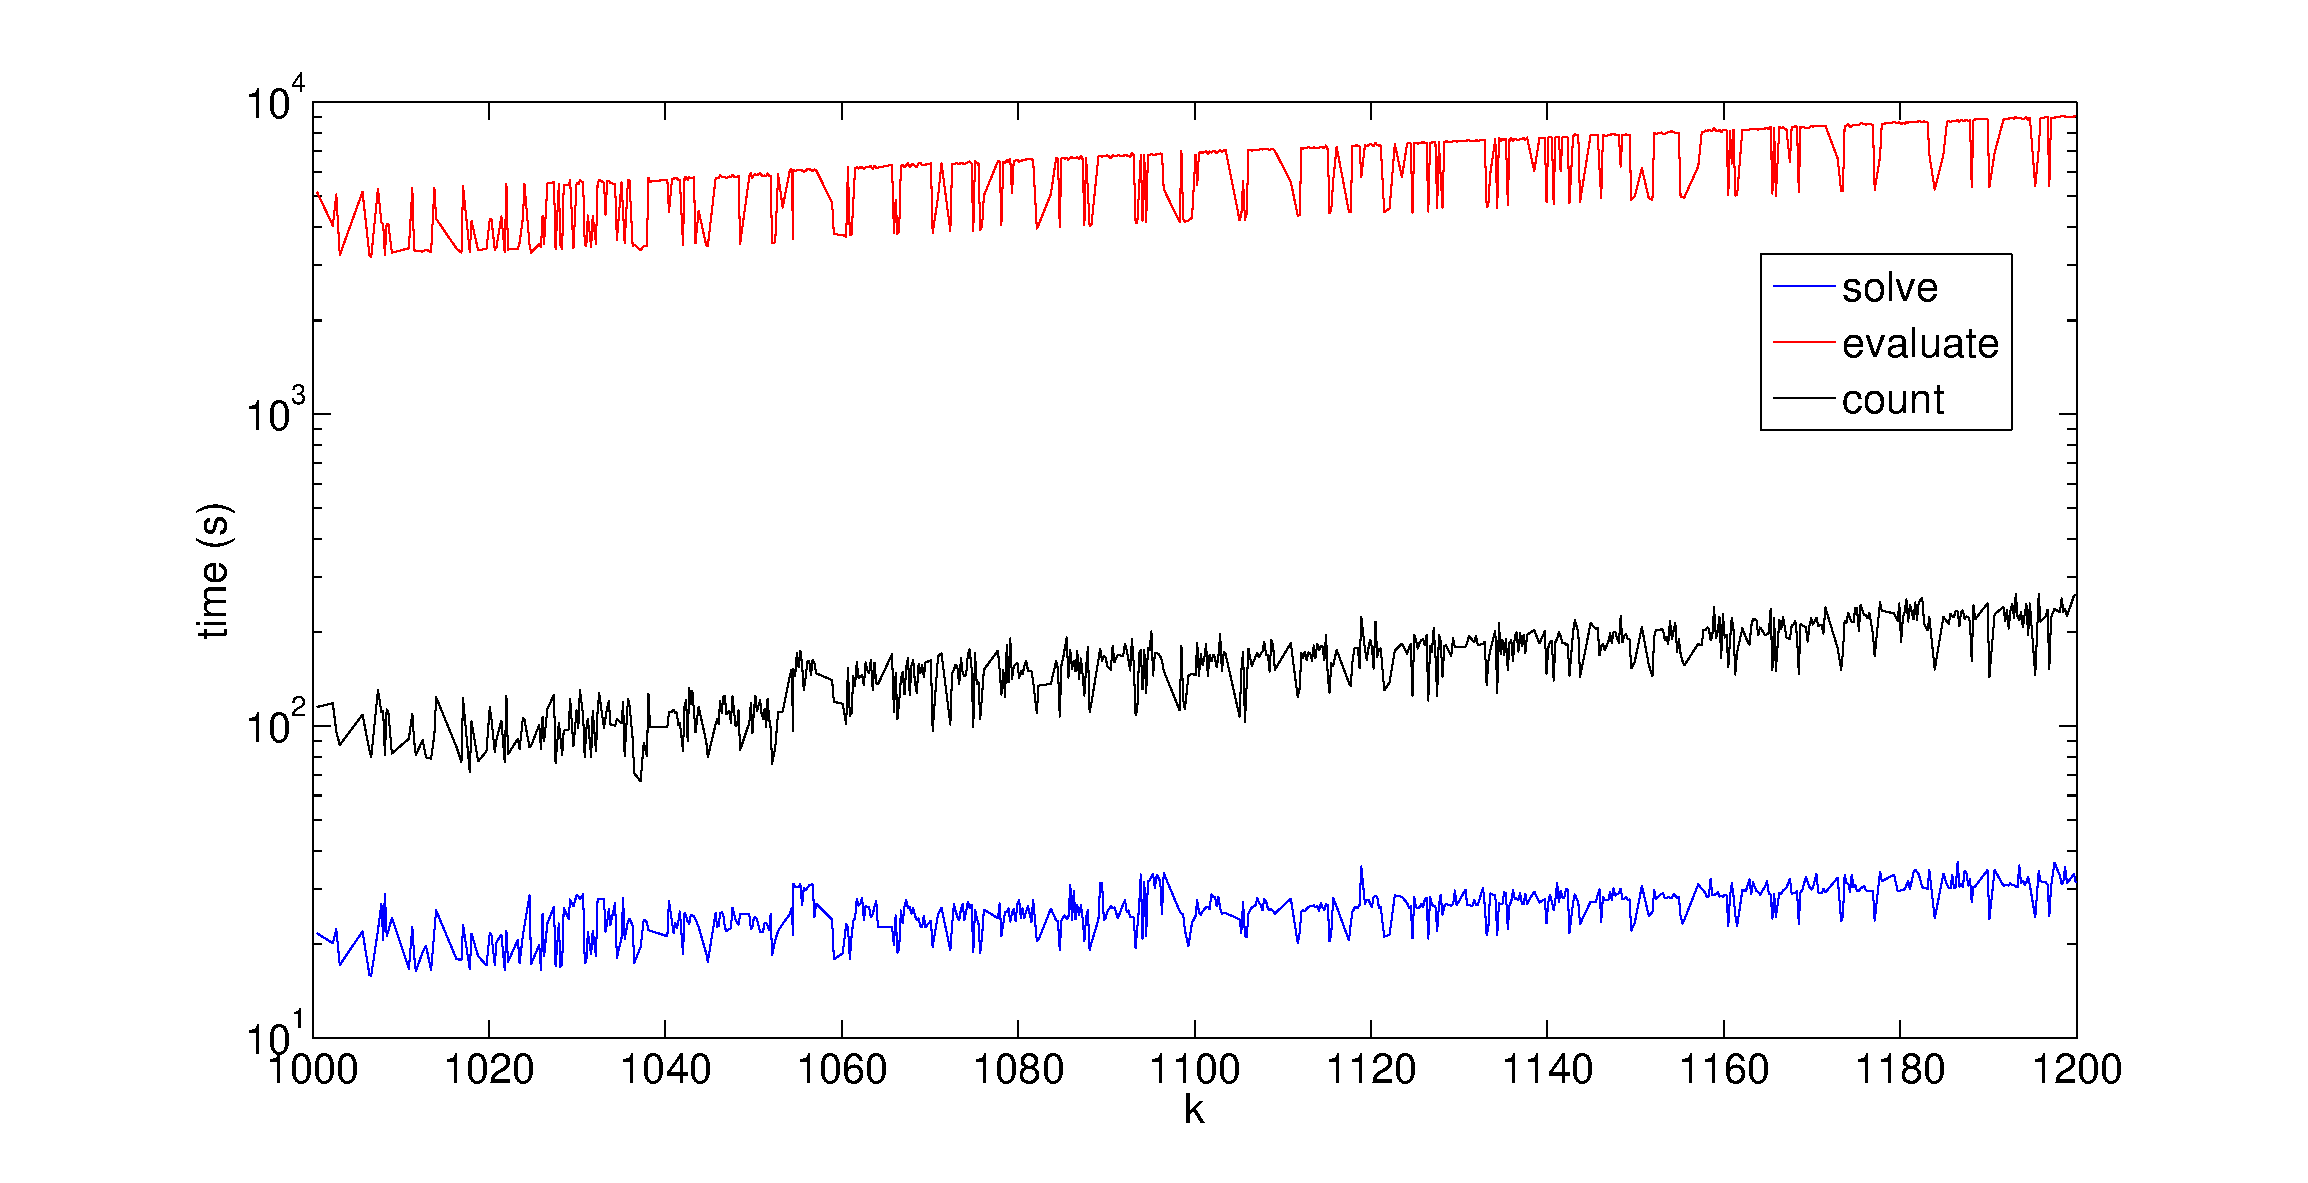
\includegraphics[width=\textwidth]{figs/timing/timing_comp_1000_to_1200.eps}
    \caption{Comparison of run times of solving for basis coefficients, evaluating eigenfunctions, and counting nodal domains. Evaluating eigenfunctions dominates runtime, taking approximately 97\% of computation time.}
    \label{fig:timing}
  \end{center}
\end{figure}


\section{Counting Nodal Domains}
Eigenfunctions are sampled on a regular grid; each point in this grid will be referred to as a ``pixel.'' Nodal domains are counted by exploring domains pixel-by-pixel, marking each pixel as ``counted'' once it has been seen. The searching algorithm usded to explore each domain is a hybrid depth- and breadth-first method where for each pixel, the sign of each neighboring pixel is compared to the sign of the nodal domain and if the sign matches, the neighboring pixel is pushed onto a stack. Exploration then continues by popping a pixel off of the stack. This method was chosen so that the signs of all four neighbors (above, below, right, and left) are known when that pixel is being examined, which is necessary for the adaptive interpolation scheme described below.

\begin{algorithm}
  \caption{Nodal domain counting algorithm}
  \begin{algorithmic}
    \Require $grid$ is $ny$ by $nx$ matrix containing eigenfunction values on billiard
    \Require $\alpha = k h$, $M$ is highest order Bessel function to interpolate with, $\rho$ is ratio to interpolate by

    \item[]
    \Function{CountNodalDomains}{$grid, \alpha, M, \rho$}
        \For{$i \in 1 \ldots ny$}
            \For{$j \in 1\ldots nx$}
                \State $counted[i][j] \gets UNCOUNTED$
            \EndFor
        \EndFor
        \State $interp \gets CreateInterpMatrix(\alpha, M, \rho)$
        \State $i,j,domains \gets 0$
        \While{$i, j \gets FindNextUnseen(counted, i, j)$}
            \State $domains \gets domains + 1$
            \State $FindDomain(grid, counted, i, j, domain\_num, interp)$
        \EndWhile
        \Return $domains$
    \EndFunction

    \item[]
    \Function{FindNextUnseen}{$counted, y, x$}
        \For{$i \in y \ldots ny$}
            \For{$j \in 1\ldots nx$}
                \If{$i=y$ and $j \leq x$}
                    \State continue
                \EndIf
                \If{$counted[i][j] = UNCOUNTED$}
                    \State \Return $i,j$
                \EndIf
            \EndFor
        \EndFor
        \State \Return $NULL$
    \EndFunction
    \algstore{count}
  \end{algorithmic}
\end{algorithm}

\clearpage
\begin{algorithm}
  \ContinuedFloat
  \caption{Nodal domain counting algorithm (continued)}
  \begin{algorithmic}
    \algrestore{count}

    \Function{FindDomain}{$grid, counted, i, j, interp$}
        \State $s.push(j,i)$
        \Comment $s$ is a stack
        \While{$x,y \gets s.pop()$}
            \State $sign \gets sign(grid[y][x])$
            \If{$InGrid(x-1,y)$}
                \If{$sign(grid(x-1,y)) = sign$}
                    \State $left \gets TRUE$
                    \If{$counted[x-1][y] = UNCOUNTED$}
                        \State $s.push(x-1,y)$
                    \EndIf
                \EndIf
            \EndIf
            \State $\ldots$ \Comment Same for $above$, $right$, and $below$

%            \If{$InGrid(x,y-1)$}
%                \If{$sign(grid(x,y-1)) = sign$}
%                    \State $above \gets TRUE$
%                    \If{$counted[x][y-1] = UNCOUNTED$}
%                        \State $s.push(x,y-1)$
%                    \EndIf
%                \EndIf
%            \EndIf
%            \If{$InGrid(x+1,y)$}
%                \If{$sign(grid(x+1,y)) = sign$}
%                    \State $right \gets TRUE$
%                    \If{$counted[x+1][y] = UNCOUNTED$}
%                        \State $s.push(x+1,y)$
%                    \EndIf
%                \EndIf
%            \EndIf
%            \If{$InGrid(x,y+1)$}
%                \If{$sign(grid(x,y+1)) = sign$}
%                    \State $below \gets TRUE$
%                    \If{$counted[x][y+1] = UNCOUNTED$}
%                        \State $s.push(x,y+1)$
%                    \EndIf
%                \EndIf
%            \EndIf

            \If{$InGrid(x-1,y-1)$ and $above$ and $left$}
                \If{$sign(grid(x-1,y-1)) = sign$}
                  \If{not $IsInterpolated(counted, x-1,y-1)$}
                      \State $Interpolate(grid, counted, x-1, y-1, interp)$
                  \EndIf
                  \If{$ConnectedAboveLeft(counted,x,y)$}
                      $s.push(x-1,y-1)$
                  \EndIf
                \EndIf
            \EndIf
            \State $\ldots$ \Comment Same for $below$ and $left$, $below$ and $right$, and $above$ and $right$
            \State $counted[y][x] = COUNTED$
        \EndWhile
    \EndFunction

  \end{algorithmic}
\end{algorithm}

Letting $N$ be the number of points the eigenfunction is sampled at, this method has computational complexity $O(N)$. This is because the method performs a fixed number of comparisons for each pixel plus $O(N)$ total comparisons searching for an unseen nodal domain after a nodal domain has been explored. This algorithm uses an array of $N$ integers to store, for each pixel, whether it has been counted, which nodal domain it is in, whether or not it is within the boundary of the billiard, and additional information relating to the interpolation method described below. In addition, this method uses a dynamically sized array as a stack whose size is (loosely) bounded above by the number of pixels in the nodal domain being explored.

\section{Interpolation}
Because sampling eigenfunctions is expensive (requiring evaluation of B = O(k) basis functions), we are limited by the total number of pixels $N$, which scales like $h^{-2}$ where $h$ is the distance between adjacent sample points, or the width and height of a pixel. As a consequence, we must work with relatively coarsely sampled eigenfunctions, causing us to encounter scenarios where the connectivity of nodal domains is ambiguous (Fig. \ref{fig:interpolation_sample}).

\begin{figure}
  \begin{center}
    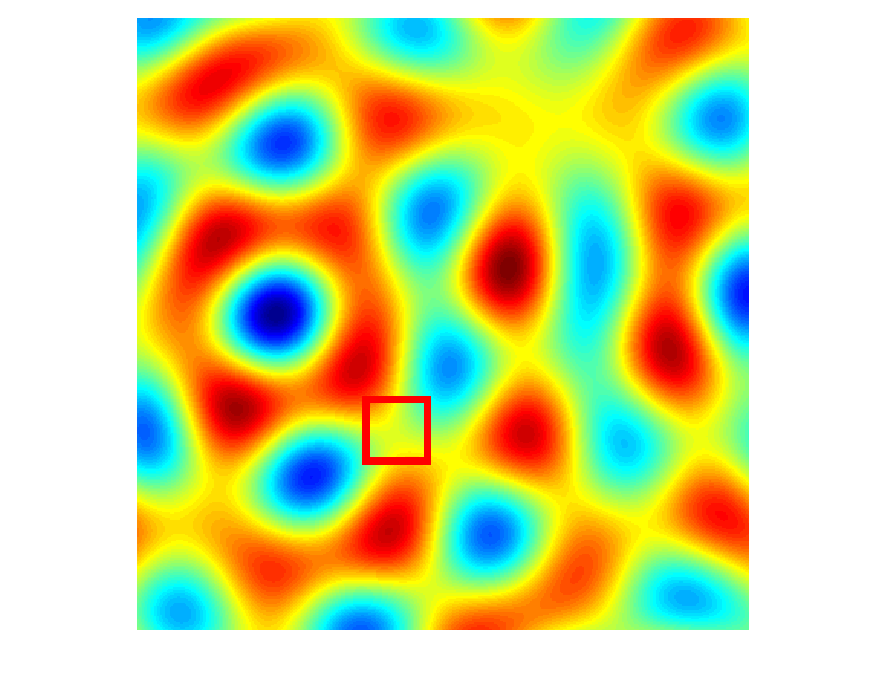
\includegraphics[width=0.49\textwidth]{figs/interpolation/interp_sample_high_res.eps}
    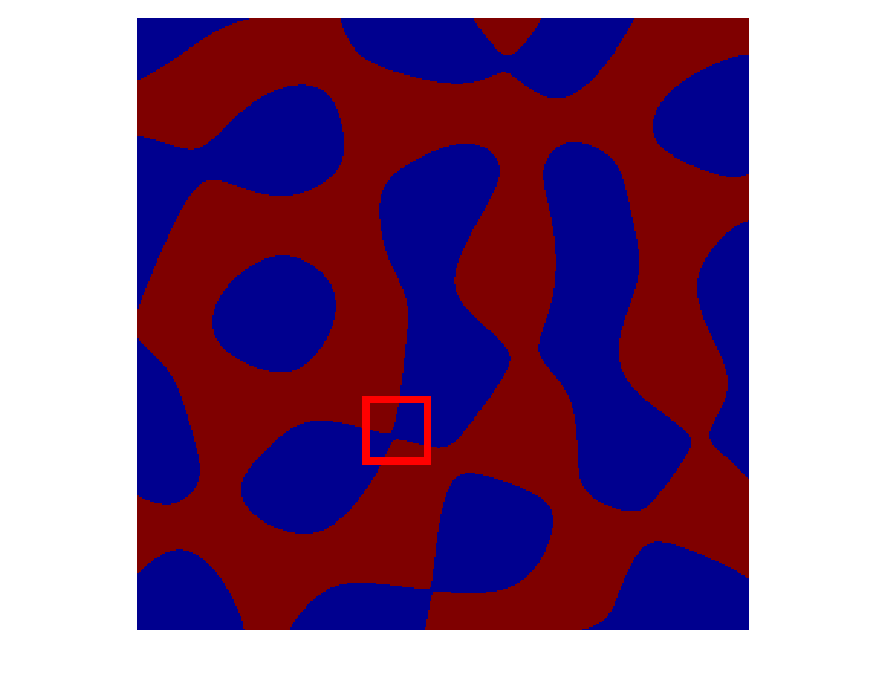
\includegraphics[width=0.49\textwidth]{figs/interpolation/interp_sample_high_res_domains.eps}
    \linebreak
    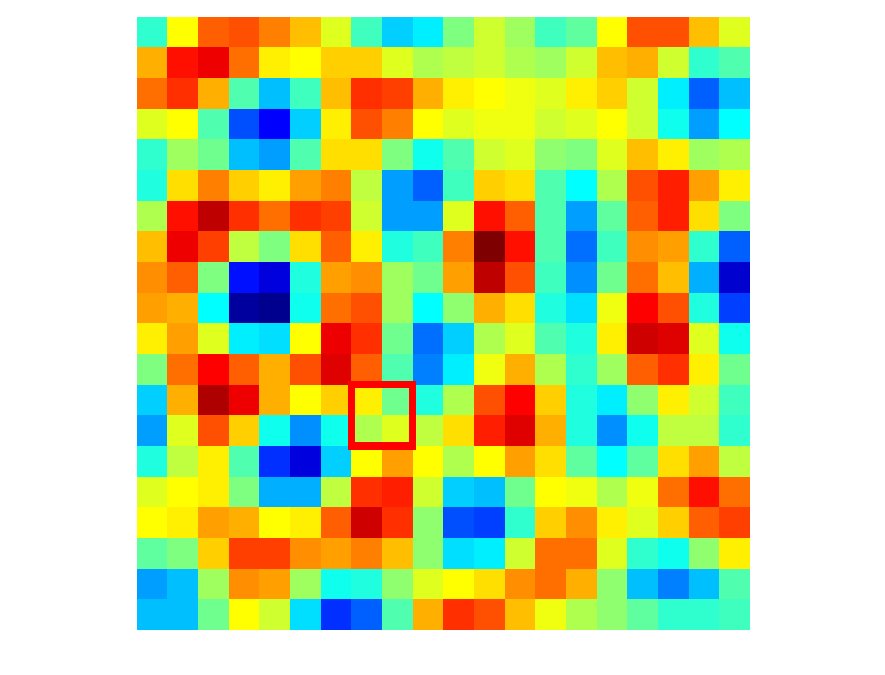
\includegraphics[width=0.49\textwidth]{figs/interpolation/interp_sample_low_res.eps}
    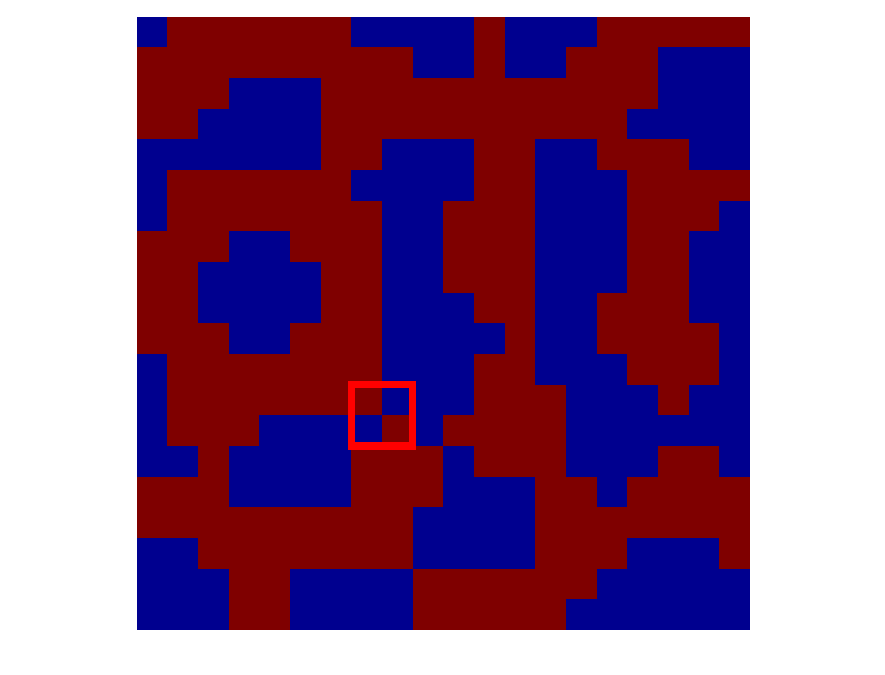
\includegraphics[width=0.49\textwidth]{figs/interpolation/interp_sample_low_res_domains.eps}

    \caption{An ambiguity in nodal domain connectivity due to coarse sampling. The ambiguous region is shown with a red box. Top left: high resolution image of an eigenfunction; top right: nodal domains of the same eigenfunction; bottom left: low resolution image of the same eigenfunction; bottom right: nodal domains of low resolution eigenfunction}
    \label{fig:interpolation_sample}
  \end{center}
\end{figure}

We resolve such ambiguities by performing an interpolation in the ambiguous region. We interpolate with the functions
\[
J_{n}(k r) \sin(n \theta)
\]
and
\[
J_{n}(k r) \cos(n \theta)
\]
where $J_{n}(r)$ is a regular Bessel function. These functions form a complete orthonormal basis for solutions of (\ref{eq:helmholtz}) (see appendix \ref{sec:helmholtz_basis}). We fix a value $M$ to be the order of the highest order Bessel function, restricting our basis to the finite set
\begin{equation}
  \label{eq:interp_functions}
  \xi_{i}(r, \theta)=\begin{cases}
  J_{i}(k r) & \text{if }i=0\\
  J_{i}(k r)\sin(i\theta) & \text{if }1 \le i \le M\\
  J_{i-M}(k r)\cos((i-M)\theta) & \text{if }M+1 \le i \le 2M
  \end{cases}
\end{equation}
We construct a surrogate function
\[
  \tilde{u}(\rr) = \sum_{i=0}^{2M} c_{i} \xi_{i}(\rr)
\]
as a local approximation to the eigenfunction $u(\rr)$ by fitting the coeffiecients $c_{i} \in \mathbb{R}$ to minimize the error $\Vert u - \tilde{u} \Vert_{2}$. This function can then be sampled at a higher resolution within the region in question. We define the sampling ratio of this surrogate function to the original eigenfunction to be $\rho$.

Interpolation occurs only between the central four pixels but uses surrounding values to fit the coefficients $c_i$. The selection of which surrounding values to use is termed a stencil. After testing various stencil shapes we selected one using 24 points consisting of a four by four square with two additional points on each side of the square. See \ref{sec:params} for a discussion of the choice of stencil, $M$, and $h$.

\subsection{Numerical Implementation}
We can construct a single matrix to transform values on a stencil to interpolated values in the center of the stencil, performing the process described above with a single matrix multiplication. We construct the interpolation matrix as
\[
U = L H^{+}
\]
Where $L$ is a matrix which contains evaluations of Bessel functions at low resolution, $H$ contains evalutions of Bessel functions at high resolution and $^{+}$ denotes the pseudoinverse. Specifically,
\[
L_{ij} =\begin{cases}
J_{j}(r_{i}) & \text{for } j = 0 \text{ and } 0 \le i < T\\
J_{j}(r_{i}) \sin{(j \theta_{i})} & \text{for } 1 \le j \le M \text{ and } 0 \le i < T\\
J_{j-M}(r_{i}) \cos{((j-M) \theta_{i})} & \text{for } M+1 \le j \le 2M+1 \text{ and } 0 \le i < T
\end{cases}
\]
and
\[
U_{ij} =\begin{cases}
J_{j}(r_{i}) & \text{for } j = 0 \text{ and } 0 \le i < \gamma\\
J_{j}(r_{i}) \sin{(j \theta_{i})} & \text{for } 1 \le j \le M \text{ and } 0 \le i < \gamma\\
J_{j-M}(r_{i}) \cos{((j-M) \theta_{i})} & \text{for } M+1 \le j \le 2M+1 \text{ and } 0 \le i < \gamma
\end{cases}
\]
where $T$ is the number of points in the stencil, $\gamma = (\rho + 1)^{2}$ and $(r_{i},\theta_{i})$ are points in the stencil expressed in polar coordinates.

The pseudoinverse $H^{+}$ is computed using a singular value decomposition as follows,
\[
H^{+} = V \Sigma^{+} U^{*}
\]
where $H = U^{*} \Sigma V$ is a singular value decompostion of $H$ and
\[
\Sigma^{+}_{ii} =\begin{cases}
\Sigma_{ii}^{-1} & \text{if }\Sigma_{ii} > \epsilon\\
\Sigma_{ii} & \text{otherwise}
\end{cases}
\]
where $\epsilon = \gamma \epsilon_{double} \Sigma_{11}$ where $\epsilon_{double}$ is the difference between $1$ and the smallest IEEE double precision floating point number greater than $1$. Singular values less than $\epsilon$ are considered to be zero within working precision.

\subsection{Code Implemenation}
A region is interpolated if and only if, when counting nodal domains, we encounter a point whose sign matches that of a point diagonally adjacent to it, but differs from the signs of the two points adjacent to both it and its diagonal neighbor (Fig. \ref{fig:trouble_spot}). In such a case we fill a vector ${\bf v}$ with the eigenfunction values at the stencil points surrounding the four points comprising the ambiguity. We then compute ${\bf w} = U {\bf v}$ where $U$ is the interpolation matrix described above. This vector ${\bf w}$ contains estimated eigenfunction values with a spacing of $\frac{h}{\rho}$ between the four points comprising the ambigious region. We can use these values to determine the connectivity of the nodal domains by traversing pixel-by-pixel from the top-left pixel, in the same manner as above, until we either reach the bottom-right pixel or finish exploring the nodal domain. In the former case the nodal domain containing the top-left pixel connects to the nodal domain containing the bottom-right pixel and in the latter case the nodal domain containing the top-right pixel connects to the nodal domain containing the bottom-left pixel.

\begin{figure}
  \begin{center}
    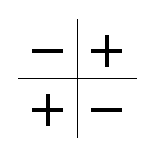
\includegraphics[width=0.2\textwidth]{figs/interpolation/trouble_spot1.eps}
    \hspace{1 cm} 
    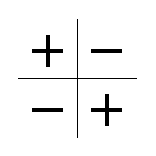
\includegraphics[width=0.2\textwidth]{figs/interpolation/trouble_spot2.eps}
    \caption{Configurations that will result in interpolation}
    \label{fig:trouble_spot}
  \end{center}
\end{figure}

\section{Code}
Code implementing Vergini's scaling method to compute eigenfunctions was written by Alex Barnett. Code for counting nodal domains was written by the author. All code used herein is open source and available under the GPL license \cite{gpl} \cite{github}. Appendix \ref{sec:api} contains an overview of the functions provided by this library.

\chapter{Results}

\section{Data Collected}
We computed approximately 100,000 eigenfunctions and counted half a billion nodal domains. This data was collected over several weeks running on the Dartmouth Mathematics Condor cluster.

\begin{table}
  \centering
  \begin{tabular}{|r|c|c|}
    \hline
    Billiard & Eigenfucntions & Nodal Domains \\ \hline
    \hline
    Sinai & 3e4 & 1.5e8 \\ \hline
    Stadium & 20 & 100 \\
    \hline
  \end{tabular}
  \caption{Ratios of basis function evaluation to multiplication for various billiards. Column $k_c$ contains the value of $k$ for which $n$ is equal to the given ratio and coefficient multiplications take as long as evaluating basis functions}
  \label{tab:results_summary}
\end{table}

\section{Mean of number of nodal domains}
We find the mean number of nodal domains to be in accordance with conjecture \ref{eq:mean_prediction}

% TODO: t-test at high k

\begin{figure}
  \begin{center}
    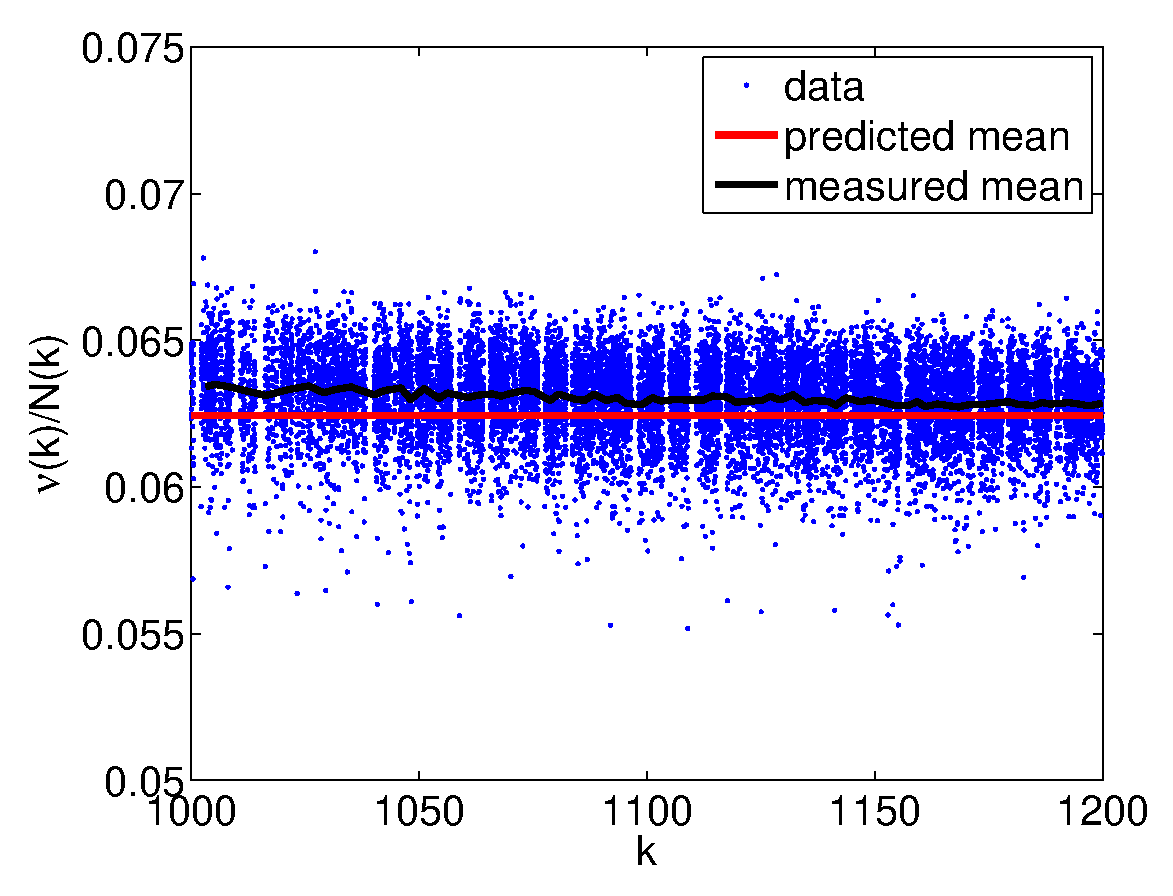
\includegraphics[width=\textwidth]{figs/results/mean.eps}
    \caption{Mean number of nodal domains}
    \label{fig:mean}
  \end{center}
\end{figure}

\section{Variance of number of nodal domains}
\begin{figure}
  \begin{center}
    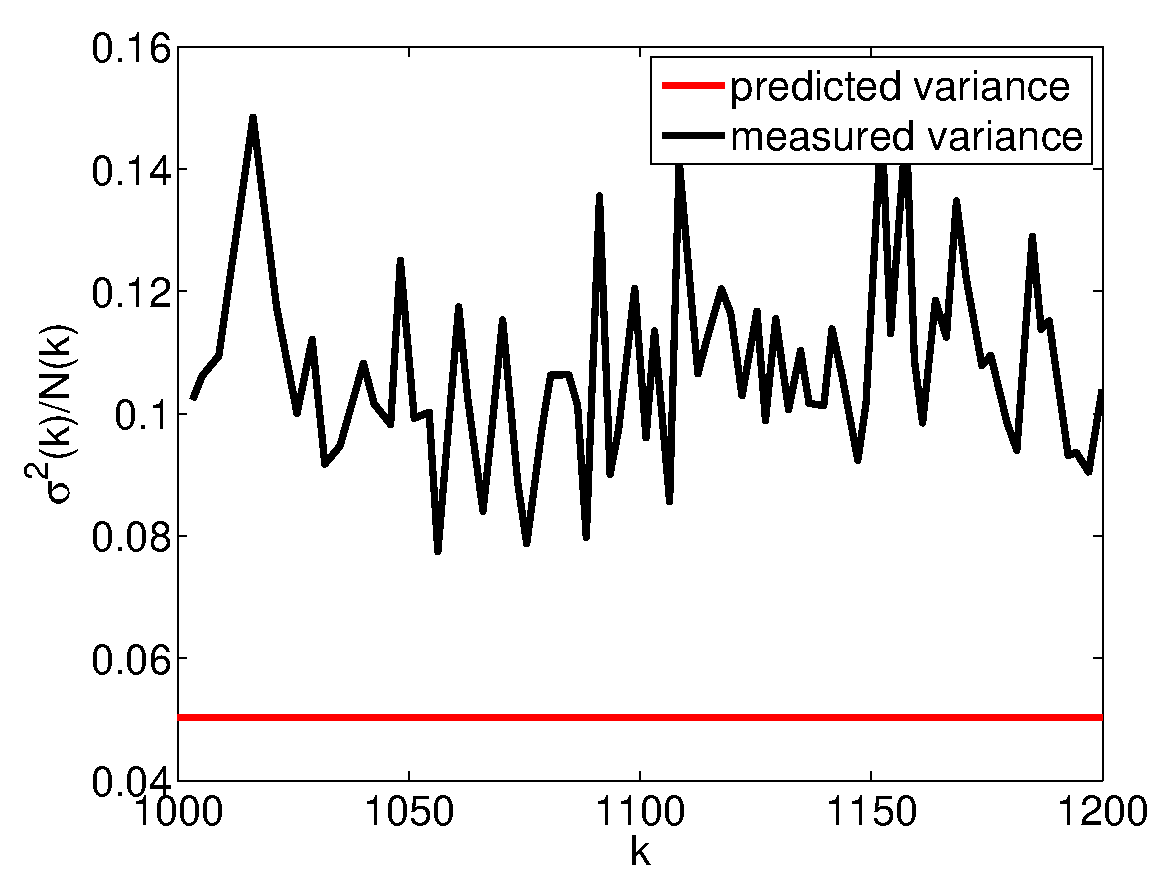
\includegraphics[width=\textwidth]{figs/results/variance.eps}
    \caption{Variance number of nodal domains}
    \label{fig:variance}
  \end{center}
\end{figure}

\section{Interpolation frequency}
At $\alpha = 0.5$ interpolation occured on average $0.1512$ times per nodal domain and $1.9e-4$ times per pixel.


% TODO: time saved by interpolating

\section{Nodal Domain Size}
\begin{figure}
  \begin{center}
    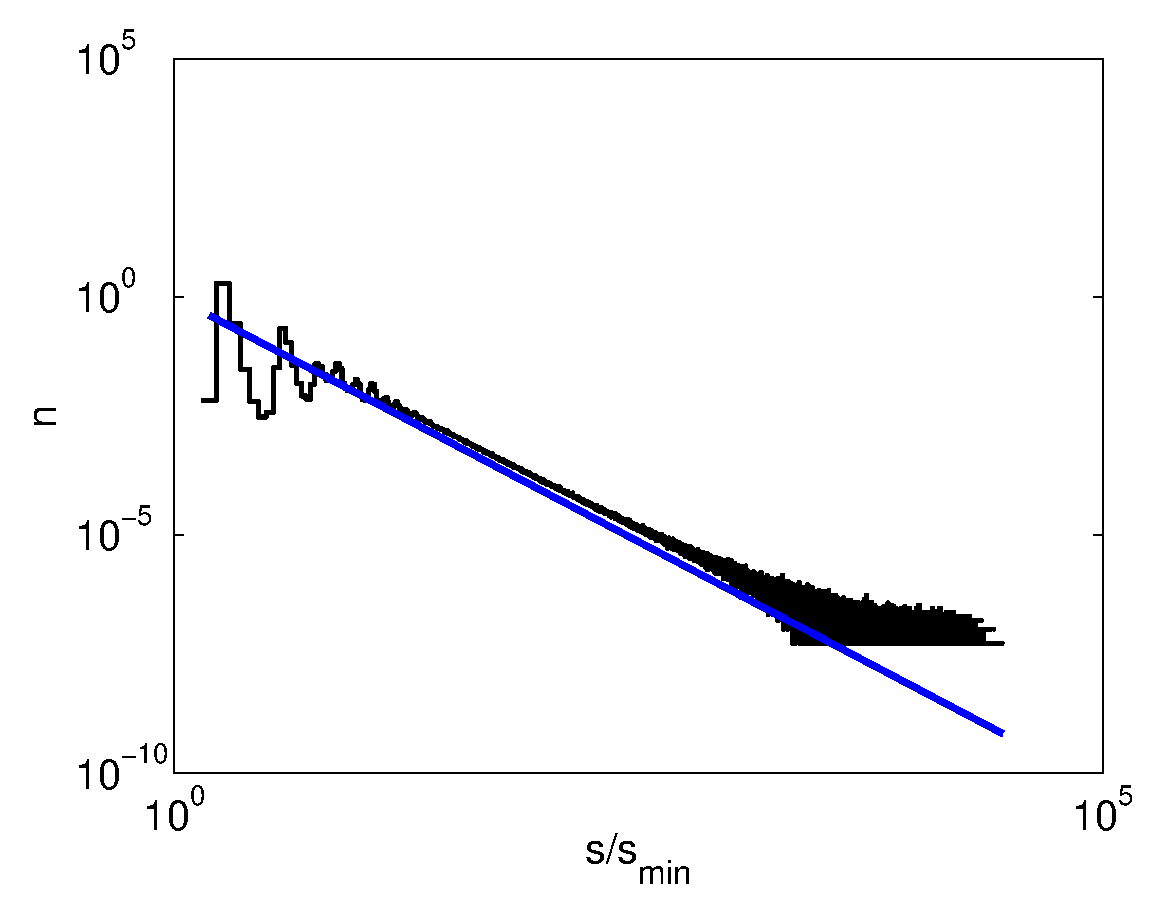
\includegraphics[width=\textwidth]{figs/results/sizes.eps}
    \caption{Size of nodal domains}
    \label{fig:sizes}
  \end{center}
\end{figure}


\appendix
\chapter{Definition of Ergodicity}
\label{sec:ergodicity}

\newtheorem{dfn}{Definition}
\begin{dfn}[$\sigma$-algebra]
$\Sigma \subset 2^{\Omega}$ is a \emph{$\sigma$-algebra} over $\Omega$ if:
\begin{enumerate}
\item
$\emptyset, \Omega \in \Sigma$
\item
$\Omega \backslash A \in \Sigma \; \forall A \in \Sigma$
\item
$\cup_{i=1}^{\infty}A_{i} \in \Sigma \; \forall \left\{A_{i}\right\}_{i=1}^{\infty}\text{ such that }A_{i} \in \Sigma \forall i$
\end{enumerate}
\end{dfn}

\begin{dfn}[Measure]
$\mu$: $\Sigma \rightarrow \mathbb{R}$ is a \emph{measure} on $\Sigma$ if:
\begin{enumerate}
\item
$\mu(A) \ge 0 \; \forall A \in \Sigma$
\item
$\mu(\emptyset) = 0$
\item
\[
\mu\left(\cup_{i=1}^{\infty} A_{i} \right) = \sum_{i=1}^{\infty} \mu(A_{i})
\]
\end{enumerate}
\end{dfn}

\begin{dfn}[Measure space]
A \emph{measure space} is a triple $(\Omega, \Sigma, \mu)$ where $\Sigma$ is a $\sigma$-algebra over $\Omega$ and $\mu$ is a measure on $\Sigma$.
\end{dfn}

\begin{dfn}[Probability space]
A \emph{probability space} is a measure space $(\Omega, \Sigma, \mu)$ where $\mu(\Omega) = 1$.
\end{dfn}

\begin{dfn}[Ergodicity]
Let $(\Omega, \Sigma, \mu)$ be a probability space. A mapping $T$: $\Sigma \rightarrow \Sigma$ is \emph{ergodic} if $T(E) = E \implies \mu(E) = 0$ or $\mu(E) = 1$
\end{dfn}
  

\chapter{General Solution of the Helmholtz Equation}
\label{sec:helmholtz_basis}
Here we show that the functions $J_{n}(k r) \sin(n \theta)$ and $J_{n}(k r) \cos(n \theta)$ form a complete orthonormal basis of solutions of (\ref{eq:helmholtz}).

In polar coordinates,
\[
\Delta = \frac{1}{r} \partial_{r} (r \partial_{r}) + \frac{1}{r^{2}} \partial_{\theta \theta}
\]
Thus, (\ref{eq:helmholtz}) can be expressed as
\[
u_{rr}(r, \theta) + \frac{1}{r} u_{r}(r, \theta) + \frac{1}{r^{2}} u_{\theta \theta}(r, \theta) + k^2 u(r, \theta) = 0
\]
Using separation of variables we attempt solutions of the form
\[
u(r, \theta) = R(r) \Theta(\theta)
\]
where $\Theta(\theta)$ is periodic with period $2 \pi$. This gives
\[
\Theta''(\theta) + n^{2} \Theta(\theta) = 0
\]
and
\[
r^{2} R''(r) + r R'(r) + r^{2} k^{2} R(r) - n^{2} R(r) = 0
\]
The periodicity of $\Theta(\theta)$ requires that
\[
\Theta(\theta) = \alpha \sin(n \theta) + \beta \cos(n \theta)
\]
where $n \in \mathbb{Z}$.
The radial differential equation is known as Bessel's equation and has solutions
\[
R(r) = J_{n}(k r)
\]
where $k \in \mathbb{R}$ is allowed to take discrete values determined by boundary conditions.

Thus, the general solution of (\ref{eq:helmholtz}) can be expressed as a sum of the form

\begin{equation}
  \label{eq:helmholtz_gen_soln}
  b_{0} J_{0}(kr) + \sum_{n = 1}^{\infty}{a_{n} J_n(kr) \sin{n \theta} + b_{n} J_n{kr} \cos{n \theta}}
\end{equation}

\chapter{Interpolation Parameter Selection}
\label{sec:params}
In this section, we discuss the various stencils, $M$, and $\alpha$ values that were considered and how we picked our particular values.
Only stencil shapes that which are symmetric about the four central points were considered. The four shapes considered are shown in figure \ref{fig:stencils}. The most important consideration in choosing a stencil was the accuracy of the interpolation. The size of the stencil affects the computational cost of interpolation but this difference is trivial.

\begin{figure}
  \begin{center}
    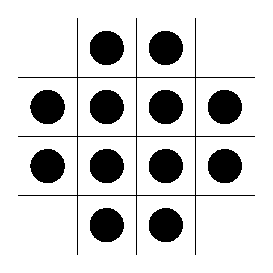
\includegraphics[width=0.2\textwidth]{figs/stencils/4x4_no_corners_centered.eps}
    \hspace{1.5 cm}
    
\includegraphics[width=0.2\textwidth]{figs/stencils/4x4_centered.eps}
    \linebreak
    \linebreak
    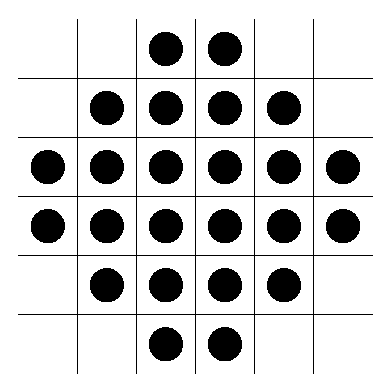
\includegraphics[width=0.3\textwidth]{figs/stencils/4x4+2_centered.eps}
    \hspace{0.4 cm}
    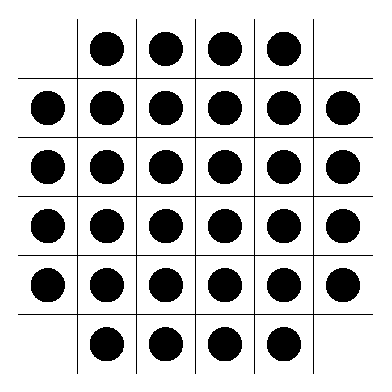
\includegraphics[width=0.3\textwidth]{figs/stencils/6x6_no_corners_centered.eps}
    \caption{The four stencil shapes considered for interpolation}
    \label{fig:stencils}
  \end{center}
\end{figure}

The accuracy of interpolation also depends on $M$ and $\alpha = k h$, which must be considered simultaneously with the choice of stencil. Figure \ref{fig:errors_all} shows a comparison of the infinity norm of the interpolation error over various values of $M$ and $\alpha$ for each of the stencils shown above.

\begin{figure}
  \begin{center}
    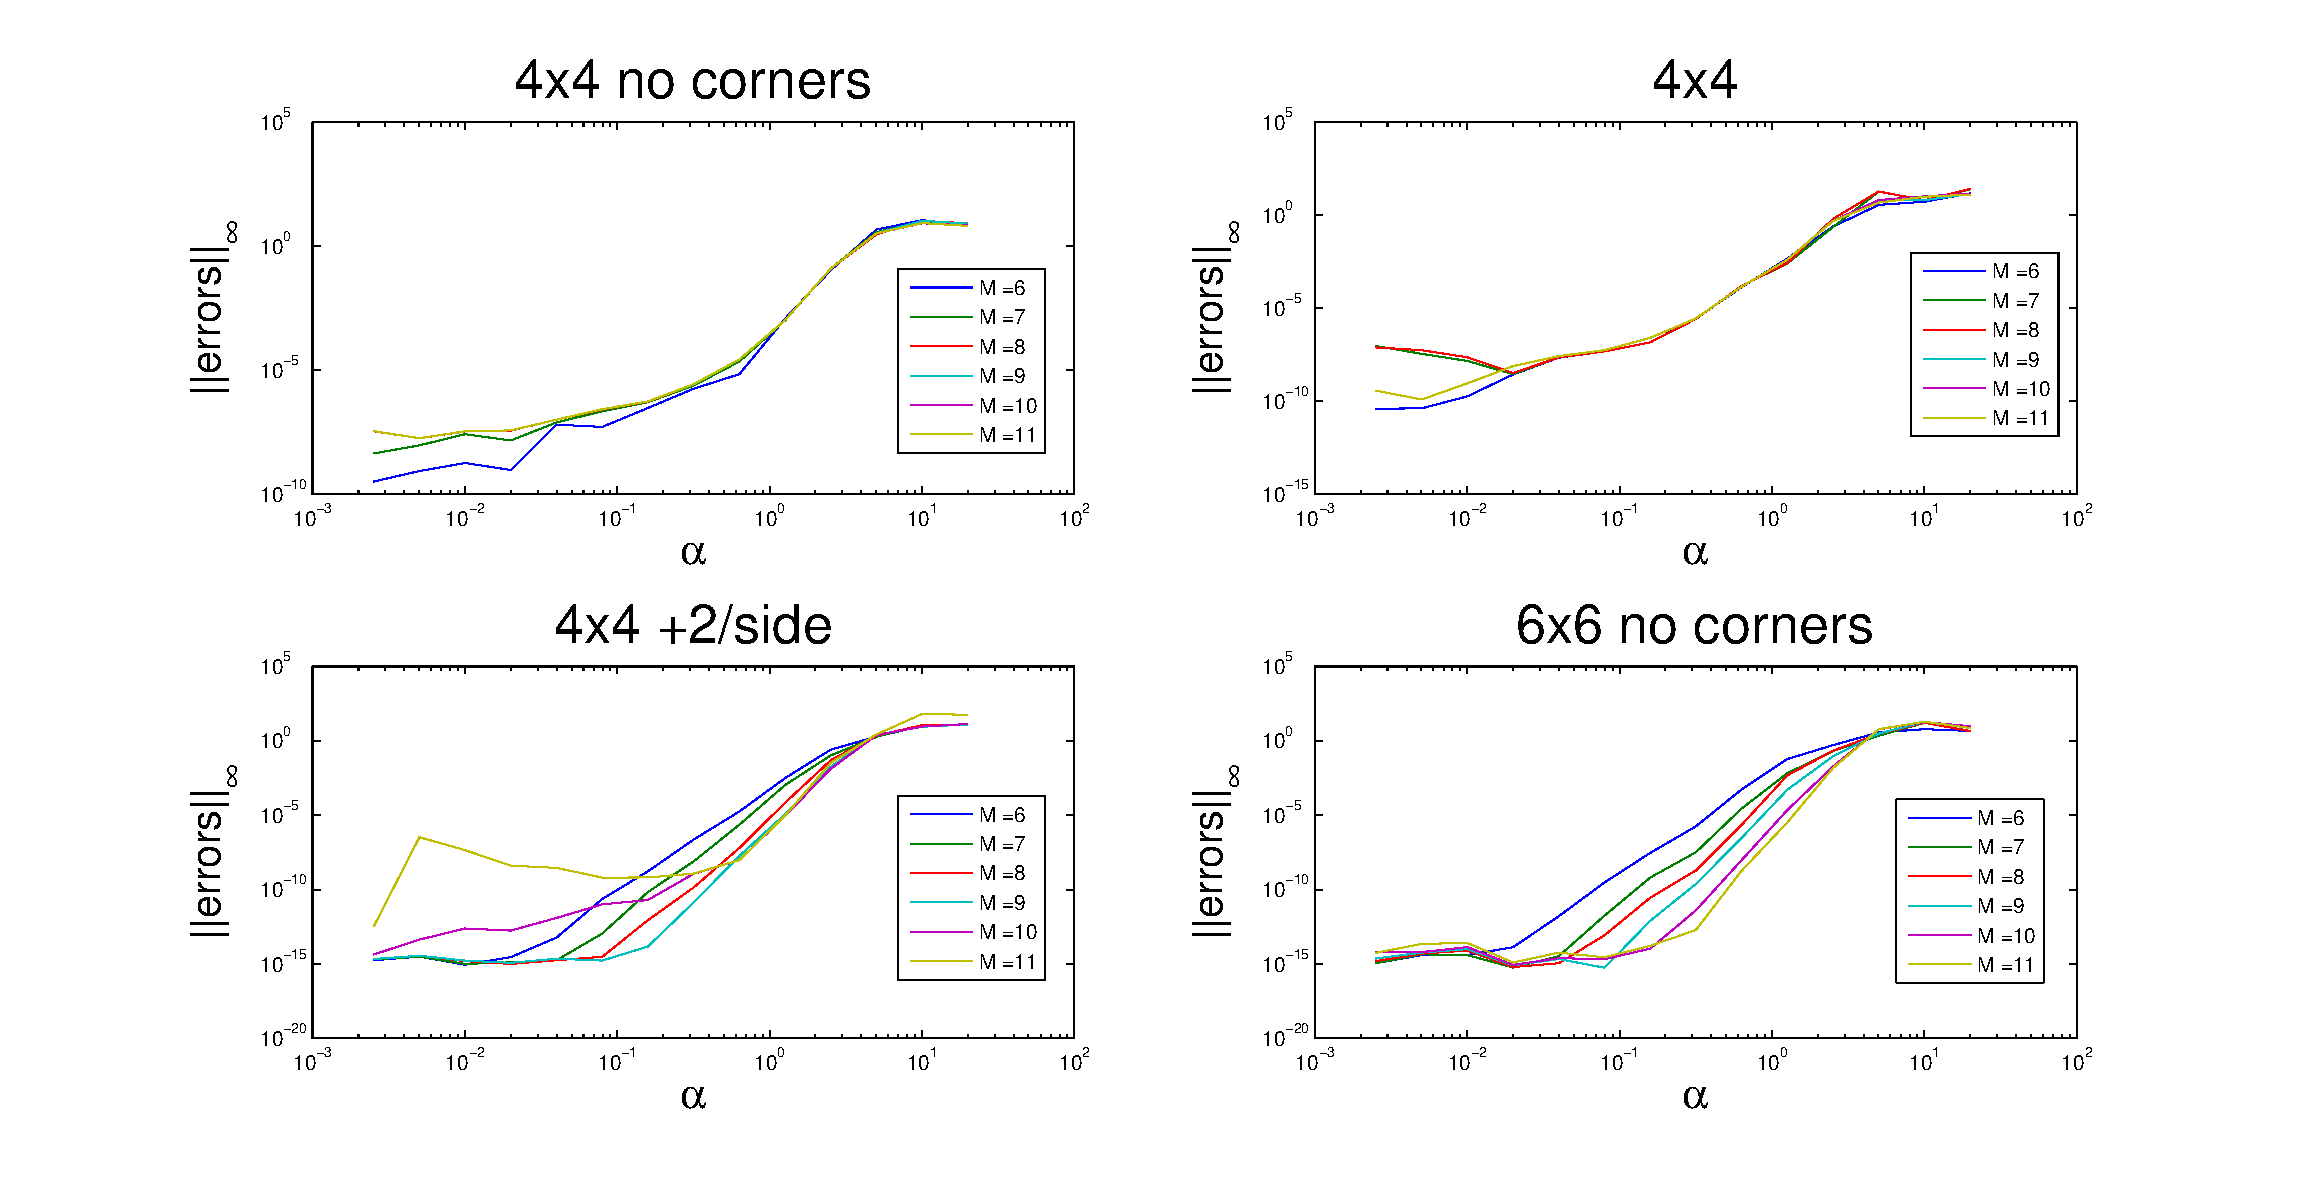
\includegraphics[width=1.2\textwidth]{figs/interpolation/error_norms_all.eps}
    \caption{Comparison of interpolation error norms over $M$ and $\alpha$ for each stencil.}
    \label{fig:errors_all}
  \end{center}
\end{figure}

\chapter{Code Interface}
\label{sec:api}
\section{Command Line Interface}
\subsection{Verg}
\begin{verbatim}
verg -l qust:2 -b 10 -s vepwoo:1.2:40:1.5 -k 200.01 -V 0.005 -f 0.001 -m
verg -l qugrs:1:0.4:0.7 -s oyooo:1.5:7:1 -u -4 1 -k 200.1 -V 0.005 -f 0.001 -m
\end{verbatim}

\subsection{Count}
\begin{verbatim}
count -f t.sta_bin -m t.mask.sta_bin -l qust:2 -d .001 -k 200.01 -M 8 -u 20
\end{verbatim}

\subsection{Vc}
\begin{verbatim}
vc -n run_2018.450000 -l qugrs:1.0:0.4:0.7 -s oyooo:1.5:7:1 -u -4 1 -k 2018.450000 -V 0.050000 -d 0.000347 -M 9 -p 30
\end{verbatim}

\subsection{Perc}
\begin{verbatim}
perc -r 100:6:1000 -N 100
\end{verbatim}


\chapter{Code Notes}
...


\bibliographystyle{plain}
\bibliography{thesis}

\end{document}
